
\documentclass{article}
\usepackage[T1]{fontenc}
\usepackage[latin2]{inputenc}
\usepackage[english]{babel}
\usepackage{tikz}
\usepackage{times}
\usetikzlibrary{calc,through,backgrounds,positioning,fit}
\usetikzlibrary{shapes,arrows,shadows}
\usetikzlibrary{calendar} 

 
 

\begin{document}

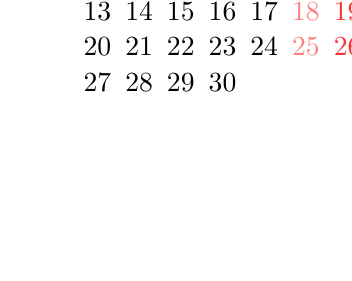
\begin{tikzpicture}

\tikz \calendar[dates=2015-04-01 to 2015-04-30,week list,
month label above centered, month text=\%mt \%y-]
if (Sunday)            [red!80]
if (Saturday)          [red!50]
if (equals=2015-04-06) [red!80];

\end{tikzpicture}

\end{document}